\chapter{EXPERIMENTAL RESULTS AND DISCUSSION}\label{ch:results}

\section{Evaluation Protocol}
All reported results are taken from the saved current 100-vehicle experiment artifacts. The held-out test set contains 300 overlapping examples, with class support of 151 free, 55 moderate and 94 heavy examples. Each method is scored against the same target rows within its comparison. Because windows overlap in time, these 300 rows are not independent observations. There is one training seed, so the values are descriptive and do not provide confidence intervals or evidence of performance stability across seeds.

Queue regression is evaluated with mean absolute error (MAE) and root mean squared error (RMSE), in metres. Congestion classification is evaluated with macro-F1 and balanced accuracy. Macro-F1 gives equal weight to each class; balanced accuracy averages per-class recall. A three-class confusion matrix is also provided to show where errors occur. The current matrices use raw counts, not row-normalized percentages.

\section{Main Results}
Table~\ref{tab:main-results} summarizes the reported comparison. The signal-aware ridge and majority baselines provide simple references. The persistence baseline is scored on the available RSU subset and therefore has fewer rows than the main 300-row comparison. The central GRU produces the strongest combined regression and classification scores in this saved run.

\begin{table}[ht]
\centering
\caption{Saved 100-vehicle evaluation metrics. Lower is better for MAE/RMSE; higher is better for macro-F1/balanced accuracy.}
\label{tab:main-results}
\small
\setlength{\tabcolsep}{3.5pt}
\begin{tabular}{lrrrrr}
\toprule
Method & Rows & MAE (m) & RMSE (m) & Macro-F1 & Bal. acc.\\
\midrule
Signal-aware ridge & 300 & 27.07 & 36.97 & 0.562 & 0.620\\
Majority class & 300 & -- & -- & 0.159 & 0.333\\
Persistence (RSU subset) & 70 & 13.80 & 28.99 & 0.557 & 0.536\\
Central GRU & 300 & 18.51 & 28.28 & 0.764 & 0.746\\
Hierarchical FL, RSU learning on & 300 & 61.48 & 68.15 & 0.342 & 0.361\\
Hierarchical FL, RSU learning off & 300 & 69.58 & 76.36 & 0.298 & 0.338\\
\bottomrule
\end{tabular}
\end{table}

\begin{figure}[ht]
\centering
\IfFileExists{figs/current_matched_metrics.png}{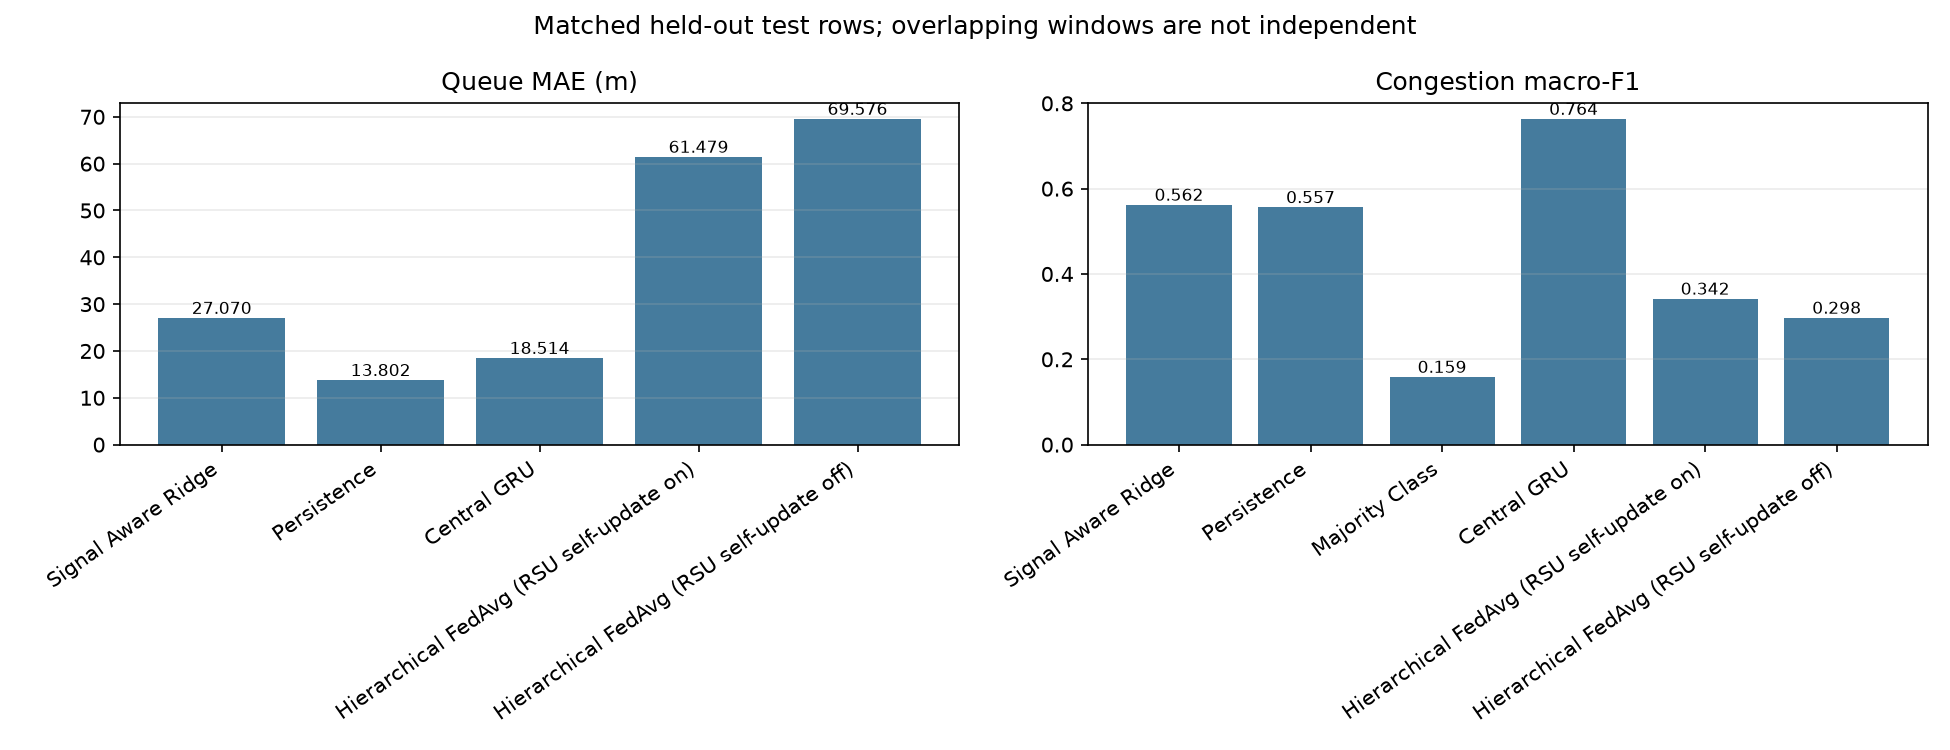
\includegraphics[width=\linewidth]{figs/current_matched_metrics.png}}{\fbox{\parbox{0.8\linewidth}{Matched-metrics figure unavailable in the source folder.}}}
\caption{Comparison of saved regression and classification metrics.}
\label{fig:metrics-current}
\end{figure}

The central model improves over the signal-aware ridge on all four listed metrics in this run. Its macro-F1 of 0.764 is notably higher than the majority baseline's 0.159, but the result should be read alongside the class support and the single-seed, overlapping-window design. The persistence row has only 70 RSU examples; its MAE should not be compared as if it had the same evaluation cohort as the 300-row methods.

\section{Central Model Training}
The central GRU's saved training record shows 50 epochs, a best validation checkpoint at epoch 35, and a run duration of 41.32 seconds (29.31 seconds of recorded training time) on CUDA. The configured minimum epoch count was 50, with a maximum of 150 and patience 15. Since training reached the minimum, early stopping did not end the run before epoch 50. Epoch 35 denotes the selected checkpoint, not the epoch at which training stopped.

\section{Federated Comparison}
The RSU-learning-enabled hierarchical run reports MAE 61.48 m and macro-F1 0.342; disabling RSU local learning reports MAE 69.58 m and macro-F1 0.298. The enabled condition is numerically better on all four metrics in this run, but this is not an isolated causal estimate of RSU learning: it includes four additional learning clients and 300 additional training windows. Both conditions use 100 rounds, five local epochs, and the same 100 configured vehicle clients, with the same held-out evaluation cohort.

Recorded wall durations were 1,056.55 seconds for RSU learning on and 1,002.25 seconds for RSU learning off. These are run-specific durations on the recorded environment; they are not a hardware-independent training-time comparison. The result also shows that the present hierarchical setup does not yet match central training quality. Possible contributors include non-IID client data, the small number of training seeds, client/aggregation dynamics, and the current training schedule. The saved experiment does not establish which factor dominates.

\section{Class-Level Errors}
Figure~\ref{fig:confusion-current} shows the current raw-count confusion matrices. The held-out support is imbalanced, with fewer moderate examples. Central GRU correct predictions are 138 free, 29 moderate, and 75 heavy. For hierarchical learning with RSU learning on, the diagonal counts are 63, 5 and 54; with RSU learning off, they are 41, 4 and 63. These raw counts make the small moderate-class diagonal appear faint in a shared color scale; percentages would answer a different question (per-class recall) and are not the values shown in this report.

\begin{table}[ht]
\centering
\caption{Class-level recall and precision derived from the saved confusion counts.}
\label{tab:class-metrics}
\small
\begin{tabular}{llrrr}
\toprule
Model & Measure & Free & Moderate & Heavy\\
\midrule
Central GRU & Recall & 0.914 & 0.527 & 0.798\\
 & Precision & 0.802 & 0.744 & 0.843\\
HFL, RSU learning on & Recall & 0.417 & 0.091 & 0.574\\
 & Precision & 0.594 & 0.263 & 0.309\\
HFL, RSU learning off & Recall & 0.272 & 0.073 & 0.670\\
 & Precision & 0.577 & 0.267 & 0.294\\
\bottomrule
\end{tabular}
\end{table}

The per-class results clarify the aggregate scores. The central GRU identifies free and heavy examples relatively well but has lower moderate recall (0.527). Both federated models have particularly low moderate recall in this held-out split. The RSU-learning-off model has higher heavy recall than free or moderate recall, consistent with its tendency to predict heavy more often. These values are calculated from the 300-row confusion matrices and are specific to the saved test set; they are not population estimates.

The user-facing raw-count view is retained to match the current report artifacts. A row-normalized visualization would put each actual class on a 0--100\% scale and emphasize recall, but would no longer show sample counts. Both views can be useful; this report's table provides per-class recall alongside counts to keep sample size visible.

\begin{figure}[ht]
\centering
\IfFileExists{figs/current_confusion_matrices.png}{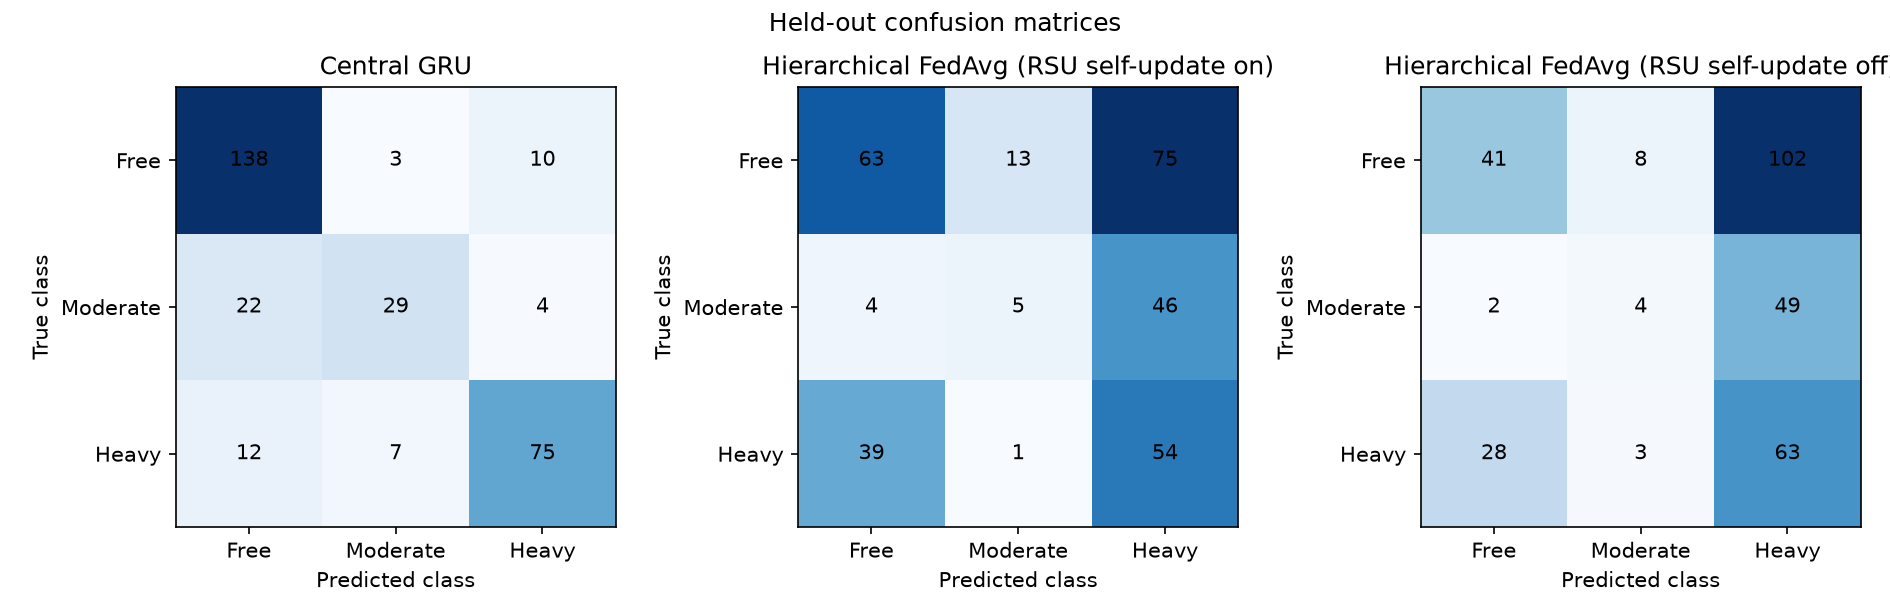
\includegraphics[width=\linewidth]{figs/current_confusion_matrices.png}}{\fbox{\parbox{0.8\linewidth}{Current confusion-matrix figure unavailable in the source folder.}}}
\caption{Raw-count confusion matrices for the central and hierarchical models.}
\label{fig:confusion-current}
\end{figure}

\section{Discussion and Limitations}
The results support the central GRU as a useful predictive baseline for the present compact simulation, not as a validated traffic deployment. The hierarchical experiments prove that the configured training path produces evaluated models, but their scores are lower than the central run. More balanced and repeated experiments are needed before attributing this gap to a specific federation design.

The experiment covers four synthetic demand scenarios at one intersection and one held-out seed per scenario. It has 300 test windows, one model-training seed, and stride-one overlapping examples. The 100-client experiment is based on configured software clients; it does not model 100 physical devices or communication faults. No real sensor data, external intersection, attack, trust intervention, or signal-control outcome is evaluated. The dataset's class distribution and observed errors should therefore be described as properties of this simulation and split.

Natural client heterogeneity is expected because vehicles and RSUs receive different bounded observations, and clients occupy different approaches and see different demand histories. Vehicles on the same approach are not automatically independent: they share the same simulated traffic stream and intersection signal. Accordingly, the effective diversity of 100 vehicle IDs is not equivalent to 100 unrelated data sources. A useful follow-up is to report per-client sample counts and label distributions, quantify between-client divergence, and compare vehicle-only, RSU-only and mixed-client training under equalized example counts.

\section{Interpretation of Queue Forecast Errors}
Queue MAE is the average absolute distance between the predicted and reference queue lengths; an MAE of 18.51 m for the central model means an average absolute error of that size on this particular test cohort. RMSE penalizes larger misses more strongly, so the central model's 28.28 m RMSE being above its MAE indicates a contribution from larger errors. These measures describe continuous queue forecasts and do not tell whether a class boundary was crossed. Conversely, macro-F1 and balanced accuracy summarize classification quality but do not indicate how many metres a queue estimate missed. Reporting both task types is therefore necessary for this multi-output model.

Classification errors can arise from small queue estimation differences near a class threshold. The class label is derived from a queue-length ratio, with boundaries at 0.10 and 0.35; a modest continuous error can change a class when the target lies close to one of those boundaries. A future analysis should report regression error by true class and distance-to-boundary, in addition to the confusion matrix. That would distinguish broad forecasting error from threshold sensitivity. The present saved report does not contain that breakdown, so this explanation is a methodological interpretation rather than a measured causal account of the observed misses.

The central model's improvement over the signal-aware ridge suggests that the sequence model learned useful temporal patterns in this simulation. It does not show that recurrence is inherently superior to other architectures: no equal-budget temporal convolution or transformer comparison is included. The GRU is the implemented model and serves as the first learned reference. Likewise, the hierarchical model's weaker scores should not be read as evidence that federation itself necessarily harms prediction. The present settings differ in data allocation and contain only one training seed. A controlled follow-up should first match the training windows and local optimization budget, then vary only the aggregation or participation rule.

For an operational interpretation, the most important limitation is the observation contract. A vehicle does not directly see the entire approach queue, and its assigned RSU does not change when it exits the junction. The model predicts an approach-level future label from the local view represented in the dataset. This supports studying distributed prediction under restricted views, but it does not yet test seamless infrastructure handoff or real sensor coverage. Those system behaviours must be implemented and validated before relating these offline metrics to continuous roadside service.

The results are suitable as a reproducible starting point for the next experiment: repeat training over multiple seeds, include more held-out runs, and compare central and federated methods under matched example budgets. Additional ablations should separately vary RSU learning, client participation, local epochs and aggregation so that each effect can be interpreted.
